
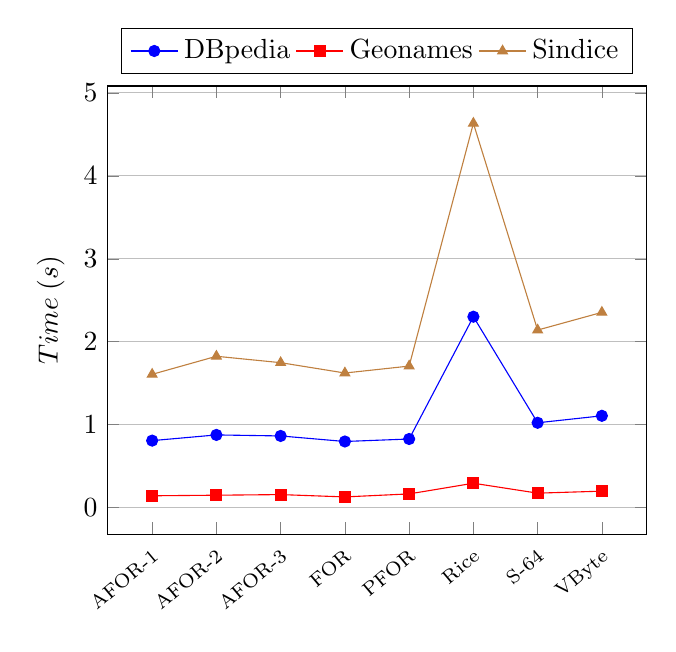
\begin{tikzpicture}
\begin{axis}[
ylabel=$Time \; (s)$,
x tick label style={font=\scriptsize, rotate=40, anchor=north east},
xtick={1,...,8},
xticklabels={AFOR-1, AFOR-2, AFOR-3, FOR, PFOR, Rice, S-64, VByte},
legend style={at={(0.5,1.13)}, anchor=north, legend columns=-1},
%ybar,
ymajorgrids=true,
%bar width=7pt,
]

\addplot[blue,mark=*]
coordinates {(1, 0.8081) (2, 0.8767) (3, 0.8644) (4, 0.7976) (5, 0.8275) (6, 2.302) (7, 1.0232) (8, 1.1072)};
\addplot[red,mark=square*]
coordinates {(1, 0.143) (2, 0.1499) (3, 0.1574) (4, 0.1293) (5, 0.1656) (6, 0.2943) (7, 0.1747) (8, 0.1988)};
\addplot[brown,mark=triangle*]
coordinates {(1, 1.6073) (2, 1.825) (3, 1.7478) (4, 1.6231) (5, 1.7067) (6, 4.6336) (7, 2.1409) (8, 2.3544)};

\legend{DBpedia, Geonames, Sindice}

\end{axis}
\end{tikzpicture}

